\subsection{Recognising the task without an instruction}
\label{sec:recogniser}

This subsection tests the recogniser \recog{} and its variant \handicap{}, which has a bound in advance (Section~\ref{sec:audit}); both read no instruction and block no task. The tests are: a feature that separates the tasks; rules that block nothing and the handicap; four zone shapes (run earlier); fresh tasks; the second benchmark and many tasks. The rule that builds zones from the inputs of a task (Section~\ref{sec:bound}) was tested first; that test, reported in Section~\ref{sec:noinstruction} at the end of this section, left a better frozen feature as the open question.
Every test was written down in the plan of the repository before it was run, with the line by which it would be read (Section~\ref{sec:protocol}); the lines are repeated below, and so are the guesses that were wrong. The exceptions are the corrected form of \handicap{} and its setting, which were chosen after numbers had been seen and are marked as such.

\paragraph{The feature.} The zone rule of Section~\ref{sec:noinstruction} (zones built from the inputs of a task; the ratio score, level 0.05, the oldest zone wins) was run with a third frozen feature: the mean of the last-layer states of the frozen T5-base encoder, without any adapter, over the tokens of the instance.
Its first test, with two other features, was run before the recogniser existed and is reported in Section~\ref{sec:noinstruction}.
Development data: the 15 SuperNI tasks of order 1, at most 400 training inputs per task, official test inputs.
Line fixed before the run: ``works'' if on average at least 90\% of the test inputs reach their own task and at most 10\% are blocked.
The guess written before was 20 to 35\% blocked.
Table~\ref{tab:recogniserfeatures} (top) shows \AudZoneFrozenTBlocked{}\% blocked and \AudZoneFrozenTOwn{}\% given to their own task, against \AudZoneSentenceBlocked{}\% and \AudZoneSentenceOwn{}\% for the sentence encoder and \AudZoneWordVecBlocked{}\% and \AudZoneWordVecOwn{}\% for the word vectors; the changed routes are \AudZoneFrozenTChanged{}\%, within the claim.
By the line the verdict is ``partial'': just below 90\% own task and just above 10\% blocked.
The guess was wrong in the good direction.
A likely reason: a sentence encoder is built to keep what a text is about and to discard how it is written, and how an input is written is most of what separates tasks.
The middle of the table shows the same lesson for a joint recogniser (Section~\ref{sec:audit}) on sentence-encoder features: adding 16 simple numbers that describe the shape of the text (length, capitals, digits, punctuation, line breaks, @, \# and web addresses) raises the share given to the own task at the end from \AudRecLrMiniEndSuperni{}\% to \AudRecLrShapeEndSuperni{}\% on the SuperNI tasks and from \AudRecLrMiniEndLong{}\% to \AudRecLrShapeEndLong{}\% on the Long Sequence tasks; character n-grams give \AudRecLrCharEndSuperni{}\% and \AudRecLrCharEndLong{}\%.

\begin{table}[t]
  \caption{Features, development data (the benchmark tasks were used to choose among the variants). Top: the zone rule of Section~\ref{sec:noinstruction} with three frozen features on the 15 SuperNI tasks; means over the tasks, in \%: test inputs inside their own zone; blocked by an older zone when their task arrives; given to their own task after the last task; whose route changed after their task arrived. Middle: a joint recogniser over all tasks, fitted by logistic regression on stored fit features or by Eq.~\eqref{eq:recogniser} on random cosine features, on the sentence encoder with or without the shape numbers or character n-grams, for the 15 SuperNI and the 15 Long Sequence tasks; the last pair of columns is $(H{+}1)/(m{+}1)$, where $H$ of the $m$ held-out inputs of a task changed route (Proposition~\ref{prop:audit}), the line against which the change was read. Bottom: the audit of Proposition~\ref{prop:audit} for the variant that was chosen (logistic regression with shape numbers): the estimate $H/m$ and the 95\% bound, averaged over the tasks.}
  \label{tab:recogniserfeatures}
  \centering
  {\footnotesize\setlength{\tabcolsep}{3pt}\begin{tabular}{lrrrr}
    \toprule
    Feature & \shortstack[r]{Inside own\\zone, \%} & \shortstack[r]{Blocked,\\\% $\downarrow$} & \shortstack[r]{Sent to\\own task\\at the end,\\\% $\uparrow$} & \shortstack[r]{Route\\changed,\\\% $\downarrow$} \\
    \midrule
    word vectors & \AudZoneWordVecInside{} & \AudZoneWordVecBlocked{} & \AudZoneWordVecOwn{} & \AudZoneWordVecChanged{} \\
    sentence encoder & \AudZoneSentenceInside{} & \AudZoneSentenceBlocked{} & \AudZoneSentenceOwn{} & \AudZoneSentenceChanged{} \\
    frozen T5-base states & \AudZoneFrozenTInside{} & \AudZoneFrozenTBlocked{} & \AudZoneFrozenTOwn{} & \AudZoneFrozenTChanged{} \\
    \bottomrule
\end{tabular}}
\par\medskip
{\footnotesize\setlength{\tabcolsep}{1.8pt}\begin{tabular}{lrrrrrr}
    \toprule
    & \multicolumn{2}{c}{\shortstack{Sent to own task\\at the end, \% $\uparrow$}} & \multicolumn{2}{c}{\shortstack{Route changed,\\\% $\downarrow$}} & \multicolumn{2}{c}{\shortstack{Audit\\$(H{+}1)/(m{+}1)$, \%}} \\
    \cmidrule(lr){2-3}\cmidrule(lr){4-5}\cmidrule(l){6-7}
    Recogniser, feature & SuperNI & Long & SuperNI & Long & SuperNI & Long \\
    \midrule
    logistic reg., sentence enc., $C=$\AudRecLrMiniParam{} & \AudRecLrMiniEndSuperni{} & \AudRecLrMiniEndLong{} & \AudRecLrMiniChangedSuperni{} & \AudRecLrMiniChangedLong{} & \AudRecLrMiniAuditLineSuperni{} & \AudRecLrMiniAuditLineLong{} \\
    \textbf{\quad + shape numbers, $C=$\AudRecLrShapeParam{}} & \textbf{\AudRecLrShapeEndSuperni{}} & \textbf{\AudRecLrShapeEndLong{}} & \textbf{\AudRecLrShapeChangedSuperni{}} & \textbf{\AudRecLrShapeChangedLong{}} & \textbf{\AudRecLrShapeAuditLineSuperni{}} & \textbf{\AudRecLrShapeAuditLineLong{}} \\
    \quad + character n-grams, $C=$\AudRecLrCharParam{} & \AudRecLrCharEndSuperni{} & \AudRecLrCharEndLong{} & \AudRecLrCharChangedSuperni{} & \AudRecLrCharChangedLong{} & \AudRecLrCharAuditLineSuperni{} & \AudRecLrCharAuditLineLong{} \\
    cosine features, sentence enc., $\lambda=$\AudRecCosMiniParam{} & \AudRecCosMiniEndSuperni{} & \AudRecCosMiniEndLong{} & \AudRecCosMiniChangedSuperni{} & \AudRecCosMiniChangedLong{} & \AudRecCosMiniAuditLineSuperni{} & \AudRecCosMiniAuditLineLong{} \\
    \quad + shape numbers, $\lambda=$\AudRecCosShapeParam{} & \AudRecCosShapeEndSuperni{} & \AudRecCosShapeEndLong{} & \AudRecCosShapeChangedSuperni{} & \AudRecCosShapeChangedLong{} & \AudRecCosShapeAuditLineSuperni{} & \AudRecCosShapeAuditLineLong{} \\
    \bottomrule
\end{tabular}}
\par\medskip
{\footnotesize\setlength{\tabcolsep}{3pt}\begin{tabular}{lrrrr}
    \toprule
    & \multicolumn{2}{c}{Audit $H/m$, \%} & \multicolumn{2}{c}{95\% bound, \%} \\
    \cmidrule(lr){2-3}\cmidrule(l){4-5}
    Chosen variant & SuperNI & Long & SuperNI & Long \\
    \midrule
    logistic reg. + shape numbers, $C=$\AudRecLrShapeParam{} & \AudRecChosenAuditEstSuperni{} & \AudRecChosenAuditEstLong{} & \AudRecChosenAuditBoundSuperni{} & \AudRecChosenAuditBoundLong{} \\
    \bottomrule
\end{tabular}}

\end{table}

\paragraph{Rules that block nothing.} Development data: the 15 SuperNI tasks, at most 400 training inputs per task, 200 of them held out (half for the tasks with fewer than 400), and the official test inputs.
Table~\ref{tab:recogniserdev} gives the rules on the frozen T5-base states, standardised with the statistics of 2{,}000 instances of other SuperNI tasks (the pool of Section~\ref{sec:protocol}, not $\mathcal{B}$).
Rule written before the run: among the variants with at most 3\% changed routes, take the highest share of test inputs given to their own task after the last task; ties go to the ridge form, which stores no input.
The rule chose \recog{} with the smallest of three penalties (``ridge $1\times$'': in the code a penalty equal to the feature dimension, 768, on sums in which every task has a total weight of 200; in Eq.~\eqref{eq:recogniser} this is $\varepsilon = 768/200 = 3.84$), tied with the logistic regression.
It gives \AudDevLLamOneArrive{}\% of the test inputs to their own task right after their task arrives and \AudDevLLamOneEnd{}\% after the last task, and \AudDevLLamOneChanged{}\% of the routes change.
Our guess before the run was 95 to 99\% on the 15 tasks; it held. We also guessed 1 to 3\% changed routes; it was \AudDevLLamOneChanged{}\%.
The weights after all 15 tasks are the same for every order of arrival, up to floating-point rounding (checked with the order reversed); on the second official order and on five random orders (Table~\ref{tab:recogniserorders}) the changed routes run from \AudOrdRandTwoLChanged{}\% to \AudOrdTwoLChanged{}\%.
The audit of Proposition~\ref{prop:audit} says \AudDevLLamOneAuditEst{}\% for the average task, with a 95\% bound of \AudDevLLamOneAuditBound{}\%, next to the \AudDevLLamOneChanged{}\% that changed on the test inputs.

\begin{table}[t]
  \caption{Rules that block nothing, development data: the 15 SuperNI tasks of order 1, frozen T5-base states, official test inputs; means over the tasks, in \%. ``Own task'': test inputs given to their own task right after it arrived and after the last task. ``Route changed'': test inputs whose route after the last task differs from the route when their task arrived. Audit $H/m$ and 95\% bound: Proposition~\ref{prop:audit}, from the held-out inputs. Bound in advance: Theorem~\ref{thm:handicap} for \handicap{}, averaged over the tasks; for the zone rule, the line described in the paragraph on zones below (not a theorem of this paper). $C$: the inverse penalty of the logistic regression. Ridge $1\times$, $10\times$, $100\times$: the penalty of Eq.~\eqref{eq:recogniser} in multiples of the smallest. $r$: a new zone may hold at most $r - 1$ held-out inputs of an older task. Bold: the variants used later. The last three rows are the first form of \handicap{}, without the floor at zero in Eq.~\eqref{eq:handicap}. The rows were compared on these tasks, so these are development numbers.}
  \label{tab:recogniserdev}
  \centering
  {\scriptsize\setlength{\tabcolsep}{2.5pt}\begin{tabular}{p{1.6in}rrrrrr}
    \toprule
    Rule & \shortstack[r]{Sent to\\own task\\at arrival,\\\% $\uparrow$} & \shortstack[r]{Sent to\\own task\\at the end,\\\% $\uparrow$} & \shortstack[r]{Route\\changed,\\\% $\downarrow$} & \shortstack[r]{Audit\\$H/m$, \%} & \shortstack[r]{95\% bound,\\\%} & \shortstack[r]{Bound in\\advance, \%} \\
    \midrule
    \recog{} with logistic regression ($C = 1$) & \AudDevJCOneArrive{} & \AudDevJCOneEnd{} & \AudDevJCOneChanged{} & \AudDevJCOneAuditEst{} & \AudDevJCOneAuditBound{} & -- \\
    \textbf{\recog{}, ridge $1\times$} & \textbf{\AudDevLLamOneArrive{}} & \textbf{\AudDevLLamOneEnd{}} & \textbf{\AudDevLLamOneChanged{}} & \textbf{\AudDevLLamOneAuditEst{}} & \textbf{\AudDevLLamOneAuditBound{}} & \textbf{--} \\
    \recog{}, ridge $10\times$ & \AudDevLLamTenArrive{} & \AudDevLLamTenEnd{} & \AudDevLLamTenChanged{} & \AudDevLLamTenAuditEst{} & \AudDevLLamTenAuditBound{} & -- \\
    \recog{}, ridge $100\times$ & \AudDevLLamHundredArrive{} & \AudDevLLamHundredEnd{} & \AudDevLLamHundredChanged{} & \AudDevLLamHundredAuditEst{} & \AudDevLLamHundredAuditBound{} & -- \\
    zones, newest wins, $r = 1$ & \AudDevClaimsROneArrive{} & \AudDevClaimsROneEnd{} & \AudDevClaimsROneChanged{} & -- & -- & \AudDevClaimsROneBound{} \\
    \handicap{}, $\nu = 0$ & \AudDevHPrimeTZeroArrive{} & \AudDevHPrimeTZeroEnd{} & \AudDevHPrimeTZeroChanged{} & -- & -- & \AudDevHPrimeTZeroBound{} \\
    \handicap{}, $\nu = 1$ & \AudDevHPrimeTOneArrive{} & \AudDevHPrimeTOneEnd{} & \AudDevHPrimeTOneChanged{} & -- & -- & \AudDevHPrimeTOneBound{} \\
    \textbf{\handicap{}, $\nu = 2$} & \textbf{\AudDevHPrimeTTwoArrive{}} & \textbf{\AudDevHPrimeTTwoEnd{}} & \textbf{\AudDevHPrimeTTwoChanged{}} & \textbf{--} & \textbf{--} & \textbf{\AudDevHPrimeTTwoBound{}} \\
    \handicap{}, $\nu = 5$ & \AudDevHPrimeTFiveArrive{} & \AudDevHPrimeTFiveEnd{} & \AudDevHPrimeTFiveChanged{} & -- & -- & \AudDevHPrimeTFiveBound{} \\
    \handicap{} without protection ($\nu = \infty$) & \AudDevHPrimeTNoneArrive{} & \AudDevHPrimeTNoneEnd{} & \AudDevHPrimeTNoneChanged{} & -- & -- & -- \\
    \midrule
    \handicap{} without the floor (first form), $\nu = 0$ & \AudDevHTZeroArrive{} & \AudDevHTZeroEnd{} & \AudDevHTZeroChanged{} & -- & -- & \AudDevHTZeroBound{} \\
    \handicap{} without the floor (first form), $\nu = 1$ & \AudDevHTOneArrive{} & \AudDevHTOneEnd{} & \AudDevHTOneChanged{} & -- & -- & \AudDevHTOneBound{} \\
    \handicap{} without the floor (first form), $\nu = 2$ & \AudDevHTTwoArrive{} & \AudDevHTTwoEnd{} & \AudDevHTTwoChanged{} & -- & -- & \AudDevHTTwoBound{} \\
    \bottomrule
\end{tabular}}

\end{table}

\begin{table}[t]
  \caption{\recog{} (ridge $1\times$) and \handicap{} ($\nu = 2$) on other orders of the same 15 SuperNI tasks, development data: the second official order and five random orders. Columns as in Table~\ref{tab:recogniserdev}; $(H{+}1)/(m{+}1)$ is the line against which the changed routes were read, and the 95\% bound is the audit's.}
  \label{tab:recogniserorders}
  \centering
  {\footnotesize\setlength{\tabcolsep}{3pt}\begin{tabular}{lrrrrrrr}
    \toprule
    & \multicolumn{5}{c}{\recog{}} & \multicolumn{2}{c}{\handicap{}, $\nu = 2$} \\
    \cmidrule(lr){2-6}\cmidrule(l){7-8}
    Order & \shortstack[r]{Sent to\\own task\\at arrival,\\\% $\uparrow$} & \shortstack[r]{Sent to\\own task\\at the end,\\\% $\uparrow$} & \shortstack[r]{Route\\changed,\\\% $\downarrow$} & \shortstack[r]{$(c{+}1)/$\\$(m{+}1)$, \%} & \shortstack[r]{95\% bound,\\\%} & \shortstack[r]{Sent to\\own task\\at the end,\\\% $\uparrow$} & \shortstack[r]{Route\\changed,\\\% $\downarrow$} \\
    \midrule
    order 1 & \AudOrdOneLArrive{} & \AudOrdOneLEnd{} & \AudOrdOneLChanged{} & \AudOrdOneLAuditLine{} & \AudOrdOneLAuditBound{} & \AudOrdOneHEnd{} & \AudOrdOneHChanged{} \\
    order 2 & \AudOrdTwoLArrive{} & \AudOrdTwoLEnd{} & \AudOrdTwoLChanged{} & \AudOrdTwoLAuditLine{} & \AudOrdTwoLAuditBound{} & \AudOrdTwoHEnd{} & \AudOrdTwoHChanged{} \\
    random 0 & \AudOrdRandZeroLArrive{} & \AudOrdRandZeroLEnd{} & \AudOrdRandZeroLChanged{} & \AudOrdRandZeroLAuditLine{} & \AudOrdRandZeroLAuditBound{} & \AudOrdRandZeroHEnd{} & \AudOrdRandZeroHChanged{} \\
    random 1 & \AudOrdRandOneLArrive{} & \AudOrdRandOneLEnd{} & \AudOrdRandOneLChanged{} & \AudOrdRandOneLAuditLine{} & \AudOrdRandOneLAuditBound{} & \AudOrdRandOneHEnd{} & \AudOrdRandOneHChanged{} \\
    random 2 & \AudOrdRandTwoLArrive{} & \AudOrdRandTwoLEnd{} & \AudOrdRandTwoLChanged{} & \AudOrdRandTwoLAuditLine{} & \AudOrdRandTwoLAuditBound{} & \AudOrdRandTwoHEnd{} & \AudOrdRandTwoHChanged{} \\
    random 3 & \AudOrdRandThreeLArrive{} & \AudOrdRandThreeLEnd{} & \AudOrdRandThreeLChanged{} & \AudOrdRandThreeLAuditLine{} & \AudOrdRandThreeLAuditBound{} & \AudOrdRandThreeHEnd{} & \AudOrdRandThreeHChanged{} \\
    random 4 & \AudOrdRandFourLArrive{} & \AudOrdRandFourLEnd{} & \AudOrdRandFourLChanged{} & \AudOrdRandFourLAuditLine{} & \AudOrdRandFourLAuditBound{} & \AudOrdRandFourHEnd{} & \AudOrdRandFourHChanged{} \\
    \bottomrule
\end{tabular}}

\end{table}

Where it is weak: the tweet task (sentiment140) falls from \AudPtFourteenArrive{}\% to \AudPtFourteenEnd{}\% when the emotion task arrives (\AudPtFourteenC{} of its \AudPtFourteenM{} held-out inputs change route; audit \AudPtFourteenAuditEst{}\%, bound \AudPtFourteenBound{}\%; \AudPtFourteenChanged{}\% of its test inputs did change); the dialogue task (multi-woz) ends at \AudPtSevenEnd{}\%.
All other tasks end at 99 to 100\% (Table~\ref{tab:recogniserpertask}, at the end of this subsection).

\paragraph{\handicap{}, and a flaw in its first form.} \handicap{} (Eq.~\eqref{eq:handicap}) puts a bound known in advance on the same joint recogniser.
As first written, the threshold $\eta_k$ had no floor at zero.
When no held-out input of an older task lies near the newcomer, the threshold is then negative, and the newcomer takes inputs that even the joint recogniser gives to an older task.
For $\nu = 1$ and $2$ the first form changed more routes than no protection at all: \AudDevHTOneChanged{}\% and \AudDevHTTwoChanged{}\%, against \AudDevHPrimeTNoneChanged{}\% without protection. Our guess for the first form with $\nu = 0$ had been 97 to 99\% of the test inputs at their own task; it gave \AudDevHTZeroEnd{}\%.
The floor at zero is the correction.
It was made after seeing these numbers, on the same 15 tasks, so the numbers of the corrected rule are development numbers and no more; the proof is unchanged.
With the floor, \handicap{} gives at the end \AudDevHPrimeTZeroEnd{}\%, \AudDevHPrimeTOneEnd{}\% and \AudDevHPrimeTTwoEnd{}\% of the test inputs to their own task for $\nu = 0, 1, 2$, and changes \AudDevHPrimeTZeroChanged{}\%, \AudDevHPrimeTOneChanged{}\% and \AudDevHPrimeTTwoChanged{}\% of the routes; without protection the figures are \AudDevHPrimeTNoneEnd{}\% and \AudDevHPrimeTNoneChanged{}\%.
After seeing these numbers we chose $\nu = 2$, the smallest value within 0.2 points of the best at the end (the best was $\nu = 5$: \AudDevHPrimeTFiveEnd{}\%, with a bound of \AudDevHPrimeTFiveBound{}\%).
With $\nu = 0$ one task pays: quoref takes only about a third of its own inputs, because one held-out input of the news task sets the threshold (Remark~\ref{rem:auditlimits}(ii)).
For $\nu = 2$ the bound in advance, averaged over the tasks, is \AudDevHPrimeTTwoBound{}\%; what was measured is \AudDevHPrimeTTwoChanged{}\%.
The bound is loose, because most later tasks take nothing from most older ones, which it cannot know.

\paragraph{Zones can do it too, with the right feature.} In an earlier step, before the joint recogniser was chosen, four zone shapes were compared on the sentence encoder, under one rule: the newest zone wins, and no held-out input of an older task may lie inside a new zone, so no task is blocked.
Table~\ref{tab:shapesgrid} gives the share of test inputs that reach their own task at the end on the 15 SuperNI tasks (development data; the Long Sequence part of the grid was not computed).
The shape matters less than the feature: with the shape numbers three of the four shapes reach \AudShapeOvrShapeEnd{}\% to \AudShapePairShapeEnd{}\%, the balls fall to \AudShapePairKnnShapeEnd{}\%, and without the numbers the same three are at \AudShapeOvrMiniEnd{}\% to \AudShapePairMiniEnd{}\%.
The rule written before the grid chose one boundary per older task with the shape numbers (weight \AudShapePairShapeWeight{}): \AudShapePairShapeEnd{}\% at the end, \AudShapePairShapeChanged{}\% of the routes changed, against a line of \AudShapePairShapeBound{}\% on average. For this zone rule the line is the share of a task's test inputs outside its own zone when the task arrives, plus $r/(m+1)$ for every later task, where a new zone may hold at most $r - 1$ held-out inputs of an older task. It follows from the same rank argument as Theorem~\ref{thm:handicap}, but we use it as a line fixed in advance and do not state it as a theorem of this paper.
No guess was written down for the shapes.

\begin{table}[t]
  \caption{Four shapes of zone, development data: the 15 SuperNI tasks, the sentence encoder alone or with the 16 shape numbers (the weight of the numbers is the best of those tried). Rows: one flat boundary against everything older, one flat boundary per older task, balls around the task's inputs, boundaries curved by random cosine features. Means over the tasks, in \%: test inputs given to their own task after the last task; test inputs whose route changed. Bold: the variant chosen by the rule written before the grid.}
  \label{tab:shapesgrid}
  \centering
  {\footnotesize\setlength{\tabcolsep}{3pt}\begin{tabular}{lrrrrr}
    \toprule
    & \multicolumn{2}{c}{Sentence encoder} & \multicolumn{3}{c}{+ shape numbers} \\
    \cmidrule(lr){2-3}\cmidrule(l){4-6}
    Boundary & \shortstack[r]{Sent to\\own task\\at the end,\\\% $\uparrow$} & \shortstack[r]{Route\\changed,\\\% $\downarrow$} & \shortstack[r]{Sent to\\own task\\at the end,\\\% $\uparrow$} & \shortstack[r]{Route\\changed,\\\% $\downarrow$} & weight \\
    \midrule
    one boundary against everything & \AudShapeOvrMiniEnd{} & \AudShapeOvrMiniChanged{} & \AudShapeOvrShapeEnd{} & \AudShapeOvrShapeChanged{} & \AudShapeOvrShapeWeight{} \\
    one boundary per older task & \AudShapePairMiniEnd{} & \AudShapePairMiniChanged{} & \textbf{\AudShapePairShapeEnd{}} & \textbf{\AudShapePairShapeChanged{}} & \textbf{\AudShapePairShapeWeight{}} \\
    balls around the task's inputs & \AudShapePairKnnMiniEnd{} & \AudShapePairKnnMiniChanged{} & \AudShapePairKnnShapeEnd{} & \AudShapePairKnnShapeChanged{} & \AudShapePairKnnShapeWeight{} \\
    curved boundaries & \AudShapePairRffMiniEnd{} & \AudShapePairRffMiniChanged{} & \AudShapePairRffShapeEnd{} & \AudShapePairRffShapeChanged{} & \AudShapePairRffShapeWeight{} \\
    \bottomrule
\end{tabular}}

\end{table}

\paragraph{Fresh tasks.} Each rule of this paragraph was chosen on the 15 benchmark tasks and then read once on a batch of 30 fresh tasks that no earlier test had used (drawn at random from a collection of real tasks, instances only; at least 1{,}000 instances each, the last 200 as test inputs, and training and held-out inputs from a random part of the first 800).
Lines fixed before: the rule ``works'' if on average at least 85\% of the test inputs go to their own task, both right after their task arrives and after the last task; it ``does not'' below 70\%; between the two it is ``partial''. For the rule in which the oldest zone wins, the line also asked for at most 15\% blocked inputs, and read ``does not'' above 30\%.
For rules with a guarantee, the guarantee is ``met'' if the average changed share is at most the average bound (or, for the audit, the average $(H{+}1)/(m{+}1)$) plus two standard errors.
Table~\ref{tab:recogniserfresh} gives the rows that exist.
On the first batch the two zone rules on the sentence encoder did not work: the oldest zone wins gives \AudShapeFreshFirstOldestEnd{}\% to the own task at the end with \AudShapeFreshFirstOldestBlocked{}\% blocked (``\AudShapeFreshFirstOldestUse{}''), the newest zone wins \AudShapeFreshFirstNewestEnd{}\% (``\AudShapeFreshFirstNewestUse{}'').
On the second batch the zone rule with one boundary per older task and the shape numbers reaches \AudShapeFreshSecondEnd{}\% at the end and \AudShapeFreshSecondArrive{}\% at arrival, with \AudShapeFreshSecondChanged{}\% of the routes changed against its line of \AudShapeFreshSecondBound{}\% (see the paragraph on zones above): ``\AudShapeFreshSecondUse{}'', guarantee ``\AudShapeFreshSecondGuarantee{}''.
On the third batch the joint recogniser (logistic regression, sentence encoder and shape numbers) reaches \AudFreshThirdArrive{}\% and \AudFreshThirdEnd{}\%, with \AudFreshThirdChanged{}\% of the routes changed, audit \AudFreshThirdAuditEst{}\% and a 95\% bound of \AudFreshThirdAuditBound{}\% (line \AudFreshThirdAuditLine{}\%): ``\AudFreshThirdUse{}'', audit ``\AudFreshThirdCert{}''.
On the fourth batch \recog{} on the frozen model's states, the rule that is used for trained answers in Section~\ref{sec:nodeftrained}, reaches \AudFreshFourthLArrive{}\% at arrival and \AudFreshFourthLEnd{}\% at the end, with \AudFreshFourthLChanged{}\% of the routes changed, audit \AudFreshFourthAuditEst{}\% and a 95\% bound of \AudFreshFourthAuditBound{}\% (line \AudFreshFourthLAuditLine{}\%): ``\AudFreshFourthUse{}'', audit ``\AudFreshFourthCert{}''.
Our guess had been 80 to 90\%.
\handicap{} ($\nu = 2$), reported next to it on the same batch by a line fixed before (within 2 points of \recog{} at the end), reaches \AudFreshFourthHEnd{}\% and changes \AudFreshFourthHChanged{}\% of the routes.
The batches differ, so the rows do not compare the rules.

\begin{table}[t]
  \caption{Fresh tasks: each rule was chosen on the benchmark tasks and read once on a batch of 30 tasks that nothing had used. Rows: the rule and the batch. Columns, means over the 30 tasks, in \%: test inputs given to their own task right after their task arrived and after the last task; routes changed; audit $H/m$ and 95\% bound where the rule has an audit. Verdict: use / guarantee, by the lines in the text (works: at least 85\% own task at arrival and at the end; does not: below 70\%; else partial). The last column is the number of tasks below 70\% own task.}
  \label{tab:recogniserfresh}
  \centering
  {\scriptsize\setlength{\tabcolsep}{2pt}\begin{tabular}{p{0.95in}rrrrrcr}
    \toprule
    Fresh tasks & \shortstack[r]{Sent to\\own task\\at arrival,\\\% $\uparrow$} & \shortstack[r]{Sent to\\own task\\at the end,\\\% $\uparrow$} & \shortstack[r]{Route\\changed,\\\% $\downarrow$} & \shortstack[r]{Audit\\$H/m$, \%} & \shortstack[r]{95\% bound,\\\%} & Verdict & \shortstack[r]{Tasks below\\70\% $\downarrow$} \\
    \midrule
    first batch: zones, oldest wins, sentence encoder & -- & \AudShapeFreshFirstOldestEnd{} & \AudShapeFreshFirstOldestChanged{} & -- & -- & \AudShapeFreshFirstOldestUse{} / \AudShapeFreshFirstOldestClaim{} & -- \\
    first batch: zones, newest wins, sentence encoder & \AudShapeFreshFirstNewestArrive{} & \AudShapeFreshFirstNewestEnd{} & \AudShapeFreshFirstNewestChanged{} & -- & -- & \AudShapeFreshFirstNewestUse{} / \AudShapeFreshFirstNewestGuarantee{} & -- \\
    second batch: zones, newest wins, one boundary per older task, sentence encoder + shape numbers & \AudShapeFreshSecondArrive{} & \AudShapeFreshSecondEnd{} & \AudShapeFreshSecondChanged{} & -- & -- & \AudShapeFreshSecondUse{} / \AudShapeFreshSecondGuarantee{} & -- \\
    third batch: sentence enc. + shape numbers, logistic reg. & \AudFreshThirdArrive{} & \AudFreshThirdEnd{} & \AudFreshThirdChanged{} & \AudFreshThirdAuditEst{} & \AudFreshThirdAuditBound{} & \AudFreshThirdUse{} / \AudFreshThirdCert{} & \AudFreshThirdLow{} \\
    fourth batch: frozen T5-base states, \recog{} & \AudFreshFourthLArrive{} & \AudFreshFourthLEnd{} & \AudFreshFourthLChanged{} & \AudFreshFourthAuditEst{} & \AudFreshFourthAuditBound{} & \AudFreshFourthUse{} / \AudFreshFourthCert{} & \AudFreshFourthLow{} \\
    fourth batch: frozen T5-base states, \handicap{}, $\nu = 2$ & \AudFreshFourthHArrive{} & \AudFreshFourthHEnd{} & \AudFreshFourthHChanged{} & -- & -- & -- & -- \\
    \bottomrule
\end{tabular}}

\end{table}

The failure that belongs here is in the third batch, and it returns in the fourth.
Two tasks of the third batch are built on the same dataset (answers for a question, and a question for an answer).
Table~\ref{tab:conflictcount} (Section~\ref{sec:nodefpublished}) shows \AudConfFiveShared{} inputs of \AudConfFiveInputs{} (\AudConfFiveShare{}\%) that occur word for word in two tasks, all in this one pair, and neither of the first two batches has any (the fourth was not counted).
Each of the two tasks gets about half of its own inputs (\AudFreshThirdPairLow{}\% and \AudFreshThirdPairHigh{}\%).
This is the conflict of Proposition~\ref{prop:noinstructionprice} seen in data: \AudConfPairShare{}\% of the inputs of each of the two tasks occur word for word in the other, and on those no method without instructions can do better than split them. The rest of the two tasks' loss is not forced by this count, though their other inputs are texts of the same kind from the same dataset. The other tasks of the batch are not affected.
The fourth batch has a pair of tasks on the same reading passages too (its shared texts were not counted): under \recog{} the older one falls to about half of its inputs when the newer one arrives, and its audit shows it (about half of its held-out inputs change route); under \handicap{} the older task keeps its routes and the newer one is kept out instead. The price moves from the older task to the newer one; it does not go away.
A caveat from the independent check: in the fresh batches the test inputs are the last 200 instances read from a task file, while the held-out inputs are a random part of the first 800.
If a file is ordered, the two are not the same kind of draw, so the statements about change rest there on an assumption that is not ensured by construction; the shares given to the own task do not depend on it.

\paragraph{The second benchmark, and many tasks.} The frozen model's states are slow to compute on a CPU, so for this part they were computed on a GPU. Nothing was trained; only routes are measured.
These tasks had been used before to compare features for an earlier variant (the middle of Table~\ref{tab:recogniserfeatures}); \recog{} and its one setting had been fixed on the SuperNI tasks before it was read on them.
Line fixed before the run: \recog{} ``works on the second benchmark'' if at least 90\% of all official test inputs of the 15 Long Sequence tasks go to their own task after the last task, and ``does not'' below 75\%.
It gives \AudScaleLongThreeEnd{}\%, for both official orders, with \AudScaleLongThreeChanged{}\% of the routes changed, audit \AudScaleLongThreeAuditEst{}\% and a 95\% bound of \AudScaleLongThreeAuditBound{}\% (Table~\ref{tab:recogniserscale}): ``works'', audit ``met''.
Our guess was 94 to 98\%.
The weak tasks are two of the three entailment tasks: mnli falls to \AudScaleLongMnliEnd{}\% when rte arrives (\AudScaleLongMnliC{} of its \AudScaleLongMnliM{} held-out inputs change route) and rte gets \AudScaleLongRteEnd{}\%; under \handicap{} mnli keeps \AudScaleLongMnliHEnd{}\% and rte takes only \AudScaleLongRteHEnd{}\% of its inputs (Table~\ref{tab:recogniserlongpertask}).

The same job describes what happens with many tasks, on the three fresh batches that earlier tests had used; it is therefore a description and not a verdict.
With 30, 60 and 90 fresh tasks, and with all 120 tasks together (the two benchmarks and the 90 fresh tasks), \recog{} gives \AudScaleFreshThirtyEnd{}\%, \AudScaleFreshSixtyEnd{}\%, \AudScaleFreshNinetyEnd{}\% and \AudScaleAllHundredTwentyEnd{}\% of the test inputs to their own task (Figure~\ref{fig:recogniserscale}).
The changed routes rise to \AudScaleAllHundredTwentyChanged{}\% and the audit follows them (\AudScaleAllHundredTwentyAuditEst{}\%, bound \AudScaleAllHundredTwentyAuditBound{}\%).
\handicap{} changes about 1\% of the routes at every size (\AudScaleAllHundredTwentyHChanged{}\% with 120 tasks) and gives two to three points fewer inputs to their own task (\AudScaleAllHundredTwentyHEnd{}\%); its bound in advance says nothing at this size.
Our guess for 120 tasks was 90 to 95\%.
The two tasks built on the same texts show what the two rules do with a conflict. Under \recog{} the older one falls from \AudScalePairOlderLArrival{}\% to \AudScalePairOlderLEnd{}\% when the newer one arrives, and the newer one gets \AudScalePairNewerLEnd{}\%. Under \handicap{} the older one keeps \AudScalePairOlderHEnd{}\% and the newer one gets \AudScalePairNewerHEnd{}\%: the older task keeps what it found.
Two checks ran inside the job: the 15 SuperNI tasks reproduce the numbers computed on the CPU, and all \AudScaleFingerprintMatch{} of the \AudScaleFingerprintTotal{} downloaded task files hold the same texts as on the CPU.
A second version of the fresh sequences with one random split of all instances, made because of the caveat above, moved the shares by \AudScaleSplitMaxDiffEnd{} points or less.

\begin{table}[t]
  \caption{\recog{} and \handicap{} ($\nu = 2$) on the two benchmarks and on growing collections of tasks; frozen T5-base states computed on a GPU, routes only. Means over the tasks, in \%. The Long Sequence rows use all official test inputs and are read against a line fixed in advance; the rows with fresh tasks use batches that earlier tests had seen and are a description. Audit $H/m$ and 95\% bound: Proposition~\ref{prop:audit}.}
  \label{tab:recogniserscale}
  \centering
  {\scriptsize\setlength{\tabcolsep}{2.5pt}\begin{tabular}{p{0.85in}rrrrrrrr}
    \toprule
    & & \multicolumn{5}{c}{\recog{}} & \multicolumn{2}{c}{\handicap{}, $\nu = 2$} \\
    \cmidrule(lr){3-7}\cmidrule(l){8-9}
    Sequence & Tasks & \shortstack[r]{Sent\\to own\\task\\at\\arrival,\\\% $\uparrow$} & \shortstack[r]{Sent\\to own\\task\\at the\\end,\\\% $\uparrow$} & \shortstack[r]{Route\\changed,\\\% $\downarrow$} & \shortstack[r]{Audit\\$H/m$, \%} & \shortstack[r]{95\% bound,\\\%} & \shortstack[r]{Sent\\to own\\task\\at the\\end,\\\% $\uparrow$} & \shortstack[r]{Route\\changed,\\\% $\downarrow$} \\
    \midrule
    SuperNI order 1 & \AudScaleSuperniOneTasks{} & \AudScaleSuperniOneArrive{} & \AudScaleSuperniOneEnd{} & \AudScaleSuperniOneChanged{} & \AudScaleSuperniOneAuditEst{} & \AudScaleSuperniOneAuditBound{} & \AudScaleSuperniOneHEnd{} & \AudScaleSuperniOneHChanged{} \\
    SuperNI order 2 & \AudScaleSuperniTwoTasks{} & \AudScaleSuperniTwoArrive{} & \AudScaleSuperniTwoEnd{} & \AudScaleSuperniTwoChanged{} & \AudScaleSuperniTwoAuditEst{} & \AudScaleSuperniTwoAuditBound{} & \AudScaleSuperniTwoHEnd{} & \AudScaleSuperniTwoHChanged{} \\
    Long Sequence order 3 & \AudScaleLongThreeTasks{} & \AudScaleLongThreeArrive{} & \AudScaleLongThreeEnd{} & \AudScaleLongThreeChanged{} & \AudScaleLongThreeAuditEst{} & \AudScaleLongThreeAuditBound{} & \AudScaleLongThreeHEnd{} & \AudScaleLongThreeHChanged{} \\
    Long Sequence order 4 & \AudScaleLongFourTasks{} & \AudScaleLongFourArrive{} & \AudScaleLongFourEnd{} & \AudScaleLongFourChanged{} & \AudScaleLongFourAuditEst{} & \AudScaleLongFourAuditBound{} & \AudScaleLongFourHEnd{} & \AudScaleLongFourHChanged{} \\
    fresh batch 1 & \AudScaleFreshThirtyTasks{} & \AudScaleFreshThirtyArrive{} & \AudScaleFreshThirtyEnd{} & \AudScaleFreshThirtyChanged{} & \AudScaleFreshThirtyAuditEst{} & \AudScaleFreshThirtyAuditBound{} & \AudScaleFreshThirtyHEnd{} & \AudScaleFreshThirtyHChanged{} \\
    fresh batches 1+2 & \AudScaleFreshSixtyTasks{} & \AudScaleFreshSixtyArrive{} & \AudScaleFreshSixtyEnd{} & \AudScaleFreshSixtyChanged{} & \AudScaleFreshSixtyAuditEst{} & \AudScaleFreshSixtyAuditBound{} & \AudScaleFreshSixtyHEnd{} & \AudScaleFreshSixtyHChanged{} \\
    fresh batches 1+2+3 & \AudScaleFreshNinetyTasks{} & \AudScaleFreshNinetyArrive{} & \AudScaleFreshNinetyEnd{} & \AudScaleFreshNinetyChanged{} & \AudScaleFreshNinetyAuditEst{} & \AudScaleFreshNinetyAuditBound{} & \AudScaleFreshNinetyHEnd{} & \AudScaleFreshNinetyHChanged{} \\
    all & \AudScaleAllHundredTwentyTasks{} & \AudScaleAllHundredTwentyArrive{} & \AudScaleAllHundredTwentyEnd{} & \AudScaleAllHundredTwentyChanged{} & \AudScaleAllHundredTwentyAuditEst{} & \AudScaleAllHundredTwentyAuditBound{} & \AudScaleAllHundredTwentyHEnd{} & \AudScaleAllHundredTwentyHChanged{} \\
    \bottomrule
\end{tabular}}

\end{table}

\begin{figure}[t]
  \centering
  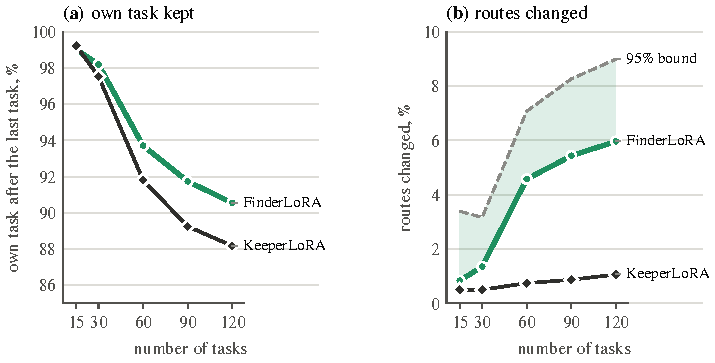
\includegraphics[width=\linewidth]{figures/recogniser_scale}
  \caption{Many tasks, routes only (frozen T5-base states). Left: share of test inputs given to their own task after the last task. Right: share of routes that changed after their task arrived, with the 95\% bound of the audit for \recog{}. The point at 15 tasks is the SuperNI benchmark; the others are 30, 60 and 90 fresh tasks and all 120 tasks together.}
  \label{fig:recogniserscale}
\end{figure}

\medskip
\noindent The per-task tables of this subsection follow.

\begin{table}[t]
  \caption{\recog{} (ridge $1\times$) per task, development data: the 15 SuperNI tasks of order 1 in the order of arrival, frozen T5-base states. Own task at arrival and at the end, route changed: \% of the test inputs of the task. Held-out: held-out inputs of the task whose route changed, of all its held-out inputs. Audit $H/m$ and 95\% bound: Proposition~\ref{prop:audit}, in \%.}
  \label{tab:recogniserpertask}
  \centering
  {\footnotesize\setlength{\tabcolsep}{3pt}\begin{tabular}{lrrrrrr}
    \toprule
    Task & \shortstack[r]{Sent to\\own task\\at arrival,\\\% $\uparrow$} & \shortstack[r]{Sent to\\own task\\at the end,\\\% $\uparrow$} & \shortstack[r]{Route\\changed,\\\% $\downarrow$} & Held-out & \shortstack[r]{Audit\\$H/m$, \%} & \shortstack[r]{95\% bound,\\\%} \\
    \midrule
    samsum & \AudPtOneArrive{} & \AudPtOneEnd{} & \AudPtOneChanged{} & \AudPtOneC{} of \AudPtOneM{} & \AudPtOneAuditEst{} & \AudPtOneBound{} \\
    sst2 & \AudPtTwoArrive{} & \AudPtTwoEnd{} & \AudPtTwoChanged{} & \AudPtTwoC{} of \AudPtTwoM{} & \AudPtTwoAuditEst{} & \AudPtTwoBound{} \\
    xsum & \AudPtThreeArrive{} & \AudPtThreeEnd{} & \AudPtThreeChanged{} & \AudPtThreeC{} of \AudPtThreeM{} & \AudPtThreeAuditEst{} & \AudPtThreeBound{} \\
    outcome extr. & \AudPtFourArrive{} & \AudPtFourEnd{} & \AudPtFourChanged{} & \AudPtFourC{} of \AudPtFourM{} & \AudPtFourAuditEst{} & \AudPtFourBound{} \\
    quoref & \AudPtFiveArrive{} & \AudPtFiveEnd{} & \AudPtFiveChanged{} & \AudPtFiveC{} of \AudPtFiveM{} & \AudPtFiveAuditEst{} & \AudPtFiveBound{} \\
    relation extr. & \AudPtSixArrive{} & \AudPtSixEnd{} & \AudPtSixChanged{} & \AudPtSixC{} of \AudPtSixM{} & \AudPtSixAuditEst{} & \AudPtSixBound{} \\
    multi-woz & \AudPtSevenArrive{} & \AudPtSevenEnd{} & \AudPtSevenChanged{} & \AudPtSevenC{} of \AudPtSevenM{} & \AudPtSevenAuditEst{} & \AudPtSevenBound{} \\
    personachat & \AudPtEightArrive{} & \AudPtEightEnd{} & \AudPtEightChanged{} & \AudPtEightC{} of \AudPtEightM{} & \AudPtEightAuditEst{} & \AudPtEightBound{} \\
    commonsenseqa & \AudPtNineArrive{} & \AudPtNineEnd{} & \AudPtNineChanged{} & \AudPtNineC{} of \AudPtNineM{} & \AudPtNineAuditEst{} & \AudPtNineBound{} \\
    diplomacy & \AudPtTenArrive{} & \AudPtTenEnd{} & \AudPtTenChanged{} & \AudPtTenC{} of \AudPtTenM{} & \AudPtTenAuditEst{} & \AudPtTenBound{} \\
    glucose & \AudPtElevenArrive{} & \AudPtElevenEnd{} & \AudPtElevenChanged{} & \AudPtElevenC{} of \AudPtElevenM{} & \AudPtElevenAuditEst{} & \AudPtElevenBound{} \\
    reddit tifu & \AudPtTwelveArrive{} & \AudPtTwelveEnd{} & \AudPtTwelveChanged{} & \AudPtTwelveC{} of \AudPtTwelveM{} & \AudPtTwelveAuditEst{} & \AudPtTwelveBound{} \\
    sciq & \AudPtThirteenArrive{} & \AudPtThirteenEnd{} & \AudPtThirteenChanged{} & \AudPtThirteenC{} of \AudPtThirteenM{} & \AudPtThirteenAuditEst{} & \AudPtThirteenBound{} \\
    sentiment140 & \AudPtFourteenArrive{} & \AudPtFourteenEnd{} & \AudPtFourteenChanged{} & \AudPtFourteenC{} of \AudPtFourteenM{} & \AudPtFourteenAuditEst{} & \AudPtFourteenBound{} \\
    emotion & \AudPtFifteenArrive{} & \AudPtFifteenEnd{} & \AudPtFifteenChanged{} & \AudPtFifteenC{} of \AudPtFifteenM{} & \AudPtFifteenAuditEst{} & \AudPtFifteenBound{} \\
    \bottomrule
\end{tabular}}

\end{table}

\begin{table}[t]
  \caption{\recog{} per task on the 15 Long Sequence tasks in order 3, all official test inputs, routes only: own task at arrival and at the end, route changed (\% of the test inputs of the task); held-out inputs whose route changed, of all; audit $H/m$ and 95\% bound (Proposition~\ref{prop:audit}); last column: own task at the end under \handicap{} ($\nu = 2$).}
  \label{tab:recogniserlongpertask}
  \centering
  {\footnotesize\setlength{\tabcolsep}{2.5pt}\begin{tabular}{lrrrrrrr}
    \toprule
    & \multicolumn{6}{c}{\recog{}} & \handicap{} \\
    \cmidrule(lr){2-7}
    Task & \shortstack[r]{Sent to\\own task\\at arrival,\\\% $\uparrow$} & \shortstack[r]{Sent to\\own task\\at the end,\\\% $\uparrow$} & \shortstack[r]{Route\\changed,\\\% $\downarrow$} & Held-out & \shortstack[r]{Audit\\$H/m$, \%} & \shortstack[r]{95\% bound,\\\%} & \shortstack[r]{Sent to\\own task\\at the end,\\\% $\uparrow$} \\
    \midrule
    yelp & \AudScaleLongPtOneArrive{} & \AudScaleLongPtOneEnd{} & \AudScaleLongPtOneChanged{} & \AudScaleLongPtOneC{} of \AudScaleLongPtOneM{} & \AudScaleLongPtOneAuditEst{} & \AudScaleLongPtOneBound{} & \AudScaleLongPtOneHEnd{} \\
    amazon & \AudScaleLongPtTwoArrive{} & \AudScaleLongPtTwoEnd{} & \AudScaleLongPtTwoChanged{} & \AudScaleLongPtTwoC{} of \AudScaleLongPtTwoM{} & \AudScaleLongPtTwoAuditEst{} & \AudScaleLongPtTwoBound{} & \AudScaleLongPtTwoHEnd{} \\
    mnli & \AudScaleLongPtThreeArrive{} & \AudScaleLongPtThreeEnd{} & \AudScaleLongPtThreeChanged{} & \AudScaleLongPtThreeC{} of \AudScaleLongPtThreeM{} & \AudScaleLongPtThreeAuditEst{} & \AudScaleLongPtThreeBound{} & \AudScaleLongPtThreeHEnd{} \\
    cb & \AudScaleLongPtFourArrive{} & \AudScaleLongPtFourEnd{} & \AudScaleLongPtFourChanged{} & \AudScaleLongPtFourC{} of \AudScaleLongPtFourM{} & \AudScaleLongPtFourAuditEst{} & \AudScaleLongPtFourBound{} & \AudScaleLongPtFourHEnd{} \\
    copa & \AudScaleLongPtFiveArrive{} & \AudScaleLongPtFiveEnd{} & \AudScaleLongPtFiveChanged{} & \AudScaleLongPtFiveC{} of \AudScaleLongPtFiveM{} & \AudScaleLongPtFiveAuditEst{} & \AudScaleLongPtFiveBound{} & \AudScaleLongPtFiveHEnd{} \\
    qqp & \AudScaleLongPtSixArrive{} & \AudScaleLongPtSixEnd{} & \AudScaleLongPtSixChanged{} & \AudScaleLongPtSixC{} of \AudScaleLongPtSixM{} & \AudScaleLongPtSixAuditEst{} & \AudScaleLongPtSixBound{} & \AudScaleLongPtSixHEnd{} \\
    rte & \AudScaleLongPtSevenArrive{} & \AudScaleLongPtSevenEnd{} & \AudScaleLongPtSevenChanged{} & \AudScaleLongPtSevenC{} of \AudScaleLongPtSevenM{} & \AudScaleLongPtSevenAuditEst{} & \AudScaleLongPtSevenBound{} & \AudScaleLongPtSevenHEnd{} \\
    imdb & \AudScaleLongPtEightArrive{} & \AudScaleLongPtEightEnd{} & \AudScaleLongPtEightChanged{} & \AudScaleLongPtEightC{} of \AudScaleLongPtEightM{} & \AudScaleLongPtEightAuditEst{} & \AudScaleLongPtEightBound{} & \AudScaleLongPtEightHEnd{} \\
    sst2 & \AudScaleLongPtNineArrive{} & \AudScaleLongPtNineEnd{} & \AudScaleLongPtNineChanged{} & \AudScaleLongPtNineC{} of \AudScaleLongPtNineM{} & \AudScaleLongPtNineAuditEst{} & \AudScaleLongPtNineBound{} & \AudScaleLongPtNineHEnd{} \\
    dbpedia & \AudScaleLongPtTenArrive{} & \AudScaleLongPtTenEnd{} & \AudScaleLongPtTenChanged{} & \AudScaleLongPtTenC{} of \AudScaleLongPtTenM{} & \AudScaleLongPtTenAuditEst{} & \AudScaleLongPtTenBound{} & \AudScaleLongPtTenHEnd{} \\
    agnews & \AudScaleLongPtElevenArrive{} & \AudScaleLongPtElevenEnd{} & \AudScaleLongPtElevenChanged{} & \AudScaleLongPtElevenC{} of \AudScaleLongPtElevenM{} & \AudScaleLongPtElevenAuditEst{} & \AudScaleLongPtElevenBound{} & \AudScaleLongPtElevenHEnd{} \\
    yahoo & \AudScaleLongPtTwelveArrive{} & \AudScaleLongPtTwelveEnd{} & \AudScaleLongPtTwelveChanged{} & \AudScaleLongPtTwelveC{} of \AudScaleLongPtTwelveM{} & \AudScaleLongPtTwelveAuditEst{} & \AudScaleLongPtTwelveBound{} & \AudScaleLongPtTwelveHEnd{} \\
    multirc & \AudScaleLongPtThirteenArrive{} & \AudScaleLongPtThirteenEnd{} & \AudScaleLongPtThirteenChanged{} & \AudScaleLongPtThirteenC{} of \AudScaleLongPtThirteenM{} & \AudScaleLongPtThirteenAuditEst{} & \AudScaleLongPtThirteenBound{} & \AudScaleLongPtThirteenHEnd{} \\
    boolq & \AudScaleLongPtFourteenArrive{} & \AudScaleLongPtFourteenEnd{} & \AudScaleLongPtFourteenChanged{} & \AudScaleLongPtFourteenC{} of \AudScaleLongPtFourteenM{} & \AudScaleLongPtFourteenAuditEst{} & \AudScaleLongPtFourteenBound{} & \AudScaleLongPtFourteenHEnd{} \\
    wic & \AudScaleLongPtFifteenArrive{} & \AudScaleLongPtFifteenEnd{} & \AudScaleLongPtFifteenChanged{} & \AudScaleLongPtFifteenC{} of \AudScaleLongPtFifteenM{} & \AudScaleLongPtFifteenAuditEst{} & \AudScaleLongPtFifteenBound{} & \AudScaleLongPtFifteenHEnd{} \\
    \bottomrule
\end{tabular}}

\end{table}
